\chapter{\label{ch:5}Nucleotide regulation of Kir6.2} 

\graphicspath{{figures/ch5/}}

\minitoc

\section{Introduction}

There are variety of ways in which mutations in Kir6.2 can lead to altered K\ATP{} channel function.
Firstly, mutations at some Kir6.2 residues can result in reduced expression of K\ATP{} at the cell membrane \cite{tornovsky_hyperinsulinism_2004, flanagan_update_2009, martin_pharmacological_2013, pipatpolkai_new_2020}.


Electrophysiological characterisation of K\ATP{} mutations tend to assign one of two roles to individual residues on Kir6.2.
Firstly, if a change in the IC\textsubscript{50} value for nucleotide inhibition is observed in the absence of a change in intrinsic (or nucleotide-independent) gating, typically measured as a change in single channel open probability (although thorough studies also tend to examine the bursting characteristics of the channel), then the residue is assumed to form part of the inhibitory nucleotide binding site but not affect transduction of binding to the channel pore.
Secondly, if a change in the IC\textsubscript{50} value for nucleotide inhibition is observed in addition to a change in intrinsic gating, the residue is assumed to regulate the relative stability of the closed and open states of the channel.
The effects on nucleotide inhibition are taken to secondary to this main effect, due to the estalished preference of nucleotides for the closed state.
Further interrogation of residues in this second category is very difficult using electrophysiological measures alone, as without measuirng binding of nucleotides directly it is impossible to truly separate effects on open probability from effects on binding and transduction.
In this chapter, we aim to clarify the role of several residues implicated in regulating the inhibitory effect of nucleotides on Kir6.2 by measuring TNP-ATP
binding directly to the inhibitory nucleotide binding site, where possible in conjunction with simultaneous current measurements.

\section{Nucleotide binding}

\subsection{G334D abolishes nucleotide binding}

Residue G334 of Kir6.2 is located in the C-terminal region (Figure \ref{ch5fig:g334d}) and has been hypothesised to form part of the ATP binding site since electrophysiological studies demonstrated a dramatic reduction in nucleotide sensitivity upon mutation of the residue \cite{drain_katp_1998, li_open_2002, li_ligand-dependent_2005}.
In addition, mutation of this residue to aspartic acid (G334D) results in severe permanent neonatal diabetes mellitus \cite{masia_atp-binding_2007-1}.
This hypothesis was confirmed by the solving of cryo-EM structures of K\ATP{} in the presence of ATP, which revealed the close proximity of residue G334 to the bound ATP \cite{lee_molecular_2017, martin_anti-diabetic_2017, li_structure_2017, puljung_cryo-electron_2018-1}.
Mutating G334 to a total of 13 different amino acid substitutions led to a increase in the IC\textsubscript{50} for ATP by over an order of magnitude in excised patches \cite{li_ligand-dependent_2005}.
However, only two of those substitutions (R and K) resulted in any changes in nucleotide-independent channel gating when examined at the single-channel level, with unliganded $P_O$ remaining constant.
It has therefore been suggested that while G334 forms part of the ATP binding site of Kir6.2, it does not participate in channel gating or transduction of ligand binding to the channel pore.

\begin{figure}[h]
	\centering
	\begin{subfigure}[t]{0.3\textwidth}
		\caption{}\label{ch5fig:g334d_loc}
		\centering
		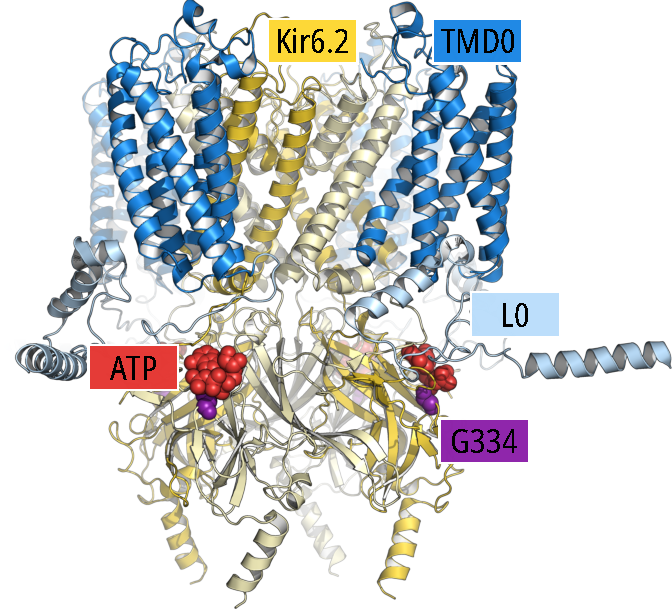
\includegraphics[width=\textwidth]{g334d_1.pdf}
	\end{subfigure}
	\hfill
	\begin{subfigure}[t]{0.5\textwidth}
		\caption{}\label{ch5fig:g334d_popfits}
		\centering
		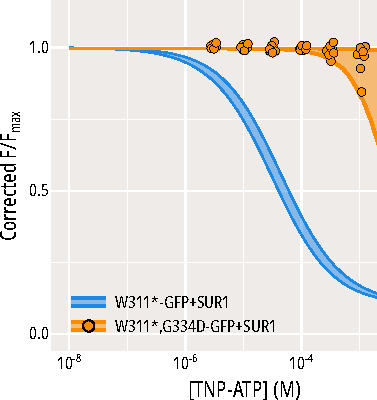
\includegraphics[width=\textwidth]{g334d_2.pdf}
	\end{subfigure}
	\vfill
	\begin{subfigure}[t]{0.9\textwidth}
		\caption{}\label{ch5fig:g334d_indfits}
		\centering
		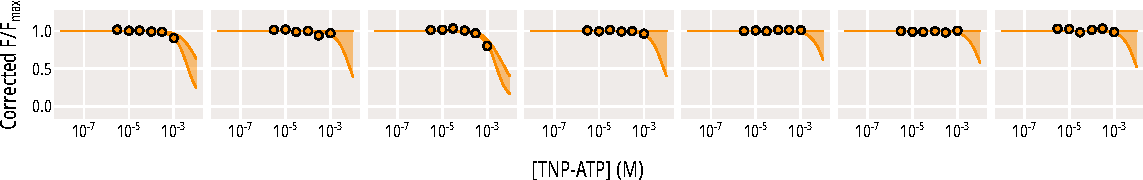
\includegraphics[width=\textwidth]{g334d_3.pdf}
	\end{subfigure}
	\vfill
	\begin{subfigure}[t]{0.45\textwidth}
		\caption{}\label{ch5fig:g334d_params}
		\centering
		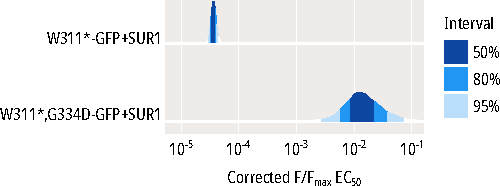
\includegraphics[width=\textwidth]{g334d_4.pdf}
	\end{subfigure}
	\caption[G334D abolishes nucleotide binding at Kir6.2]{
	\subref{ch5fig:g334d_loc} Residue G334 is shown in green in the cryo-EM structure of Kir6.2 (yellow, PDB \#6BAA).
	Docked TNP-ATP is shown as sticks in red.
	\subref{ch5fig:g334d_popfits} Fluorescence quenching of W311*,G334D-GFP+SUR1 by TNP-ATP in unroofed membrane patches.
	Each point represents an individual experiment.
	The smooth filled curves are the \SI{95}{\percent} intervals of the posterior probability distribution of fits to equation \ref{eq:hill} as described in the methods.
	\subref{ch5fig:g334d_indfits} Data from each experiment is shown separately.
	The smooth filled curves are the \SI{95}{\percent} intervals of the posterior predictions for each experiment.
	\subref{ch5fig:g334d_params} Posterior probability distributions for the estimated population $EC_{50}$ values are shown coloured according to their intervals.
	}\label{ch5fig:g334d}
\end{figure}

We sought to test this directly by measuring the binding of TNP-ATP in unroofed membranes to W311*,G334D-GFP+SUR1.
Fluorescence spectra captured from unroofed membrane patches expressing W311*,G334D-GFP+SUR1 were indistinguishable from those expressing W311*-GFP+SUR1.
The location of the ANAP peak and the bleaching characteristics were also identical.
We found that ANAP fluorescence from W311*,G334D-GFP+SUR1 was barely quenched by even \SI{1}{\milli\Molar} TNP-ATP, reducing the apparant binding EC\textsubscript{50} from \SIrange{30}{45}{\micro\Molar} to at least \SI{2.8}{\milli\Molar}.
Unfortunately, we were unable to resolve macroscopic currents from W311*,G334D-GFP+SUR1 in excised patches despite seeing fluorescence in unroofed membranes.
Thus, we were unable to measure nucleotide inhibition of this construct to determine whether the G334D substitution affected transduction in addition to this binding effect.

\section{Channel gating}

\subsection{C166S alters inhibition without affecting binding}

Residue C166 of Kir6.2 is located at the cytosolic end of the second transmembrane domain (Figure \ref{ch5fig:c166s_loc}, \cite{lee_molecular_2017, martin_anti-diabetic_2017, li_structure_2017, puljung_cryo-electron_2018-1}), and has been suggested to play a role in regulating the intrinsic gating of the channel \cite{gloyn_kcnj11_2006, trapp_molecular_1998, ribalet_atp-sensitive_2006, yang_palmitoylation_2020, loussouarn_structure_2000, enkvetchakul_kinetic_2000}.
Mutations at this residue lead to dramatically increased unliganded $P_O$ in single-channel experiments \cite{trapp_molecular_1998, enkvetchakul_kinetic_2000, ribalet_atp-sensitive_2006}, and a reduction in sensitivity to nucleotide inhibition at both single-channel and the macroscopic level \cite{trapp_molecular_1998, enkvetchakul_kinetic_2000, ribalet_atp-sensitive_2006, yang_palmitoylation_2020}.
In addition, two substitutions at this residue (F and Y) have been found to cause severe neonatal diabetes \cite{gloyn_kcnj11_2006}.
Electrophysiological measurements alone are not sufficient to distinguish between the reduction in sensitivity to nucleotide inhibition being caused by the increase in intrinsic $P_O$ alone, or whether there is an additional disregulation of transduction.

We measured TNP-ATP binding to W311*,C166S-GFP+SUR1 in unroofed membranes to determine the how mutations at C166 reduce sensitivity to nucleotide inhibition (Figure \ref{ch5fig:c166s_unroofed}).
We observed no real change in binding of TNP-ATP to the channel, with an EC\textsubscript{50} of \SIrange{44}{74}{\micro\Molar}.
If the C166S mutation solely increases the $P_O$ of the channel, we would expect an increase in the apparent EC\textsubscript{50} of nucleotide binding due to the preference of nucleotides for the closed state of the channel.
This finding suggested a role for C166 in the transduction of nucleotide binding
to the channel pore.

\begin{figure}[h]
	\centering
	\begin{subfigure}[t]{0.3\textwidth}
		\caption{}\label{ch5fig:c166s_loc}
		\centering
		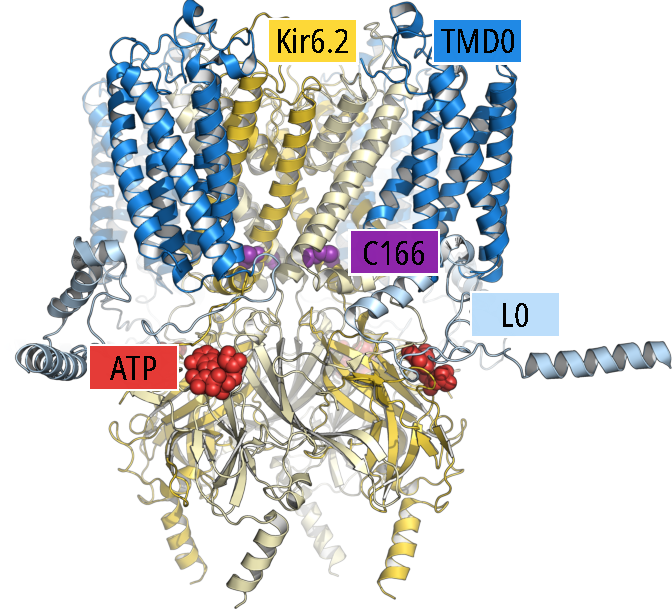
\includegraphics[width=\textwidth]{c166s_1.pdf}
	\end{subfigure}
	\hfill
	\begin{subfigure}[t]{0.5\textwidth}
		\caption{}\label{ch5fig:c166s_popfits}
		\centering
		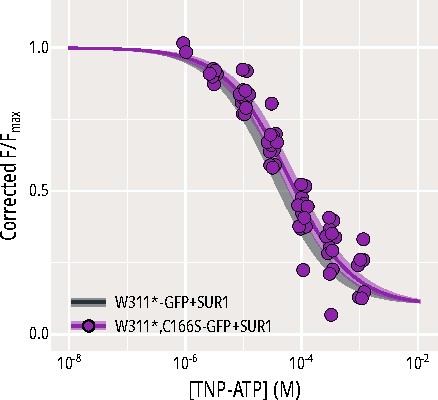
\includegraphics[width=\textwidth]{c166s_2.pdf}
	\end{subfigure}
	\vfill
	\begin{subfigure}[t]{0.9\textwidth}
		\caption{}\label{ch5fig:c166s_indfits}
		\centering
		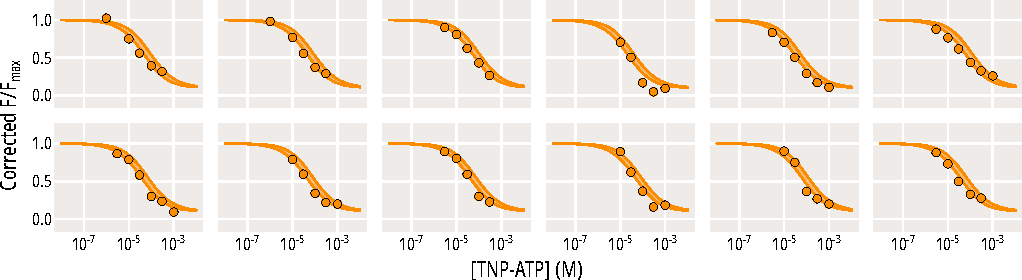
\includegraphics[width=\textwidth]{c166s_3.pdf}
	\end{subfigure}
	\vfill
	\begin{subfigure}[t]{0.45\textwidth}
		\caption{}\label{ch5fig:c166s_params}
		\centering
		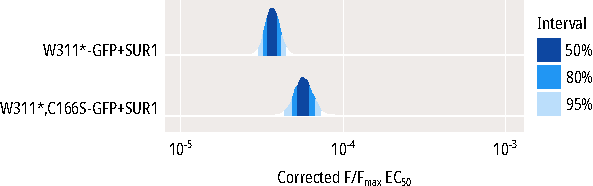
\includegraphics[width=\textwidth]{c166s_4.pdf}
	\end{subfigure}
	\caption[C166S does not alter nucleotide binding]{
	\subref{ch5fig:c166s_loc} Residue C166 is shown in purple in the cryo-EM structure of Kir6.2 (yellow, PDB \#6BAA).
	Docked TNP-ATP is shown as red spheres, and the location of W311 is shown in cyan.
	\subref{ch5fig:c166s_popfits} Fluorescence quenching of W311*,C166S-GFP+SUR1 by TNP-ATP in unroofed membrane patches.
	Each point represents an individual experiment.
	The smooth filled curves are the \SI{95}{\percent} intervals of the posterior probability distribution of fits to equation \ref{eq:hill} as described in the methods.
	\subref{ch5fig:c166s_indfits} Data from each experiment is shown separately.
	The smooth filled curves are the \SI{95}{\percent} intervals of the posterior predictions for each experiment.
	\subref{ch5fig:c166s_params} Posterior probability distributions for the estimated population $EC_{50}$ values are shown coloured according to their intervals.
	}\label{ch5fig:c166s_1}
\end{figure}

To investigate this further, we excised patches expressing W311*,C166S-GFP+SUR1 and measure current inhibition and fluorescence quenching by TNP-ATP simultaneously (Figure \ref{ch5fig:c166s_traces}).
We found that the apprent affinity for nucleotide binding was indistinguishable from that for W311*-GFP+SUR1, and similar to our observations in unroofed membranes (Figure \ref{ch5fig:c166s_mwc_fit_1}, EC\textsubscript{50} of \SIrange{26}{218}{\micro\Molar}).
Consistent with the literature, we did observe a large reduction in the apparent sensitivity of W311*,C166S-GFP+SUR1 currents to inhibition by TNP-ATP (IC\textsubscript{50} of at least \SI{155}{\micro\Molar}.
Intuitively, a change in nucleotide-dependent channel gating which is not accompanied by a change in nucleotide binding must be due (at least in part) to a change in the transduction of nucleotide binding to channel gating.

\begin{figure}[h]
	\centering
	\begin{subfigure}[t]{0.6\textwidth}
		\caption{}\label{ch5fig:c166s_traces}
		\centering
		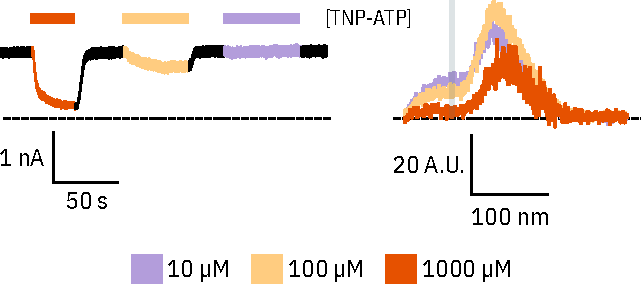
\includegraphics[width=\textwidth]{c166s_5.pdf}
	\end{subfigure}
	\hfill
	\begin{subfigure}[t]{0.3\textwidth}
		\caption{}\label{ch5fig:c166s_popfits_2}
		\centering
		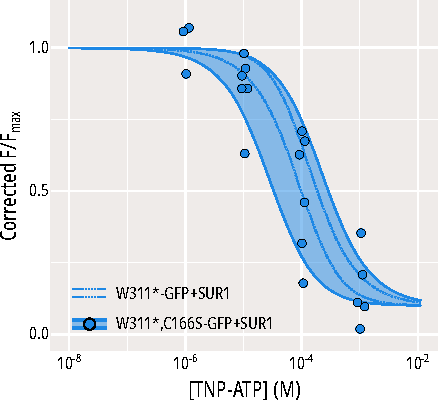
\includegraphics[width=\textwidth]{c166s_6.pdf}
	\end{subfigure}
	\vfill
	\begin{subfigure}[t]{0.3\textwidth}
		\caption{}\label{ch5fig:c166s_popfits_3}
		\centering
		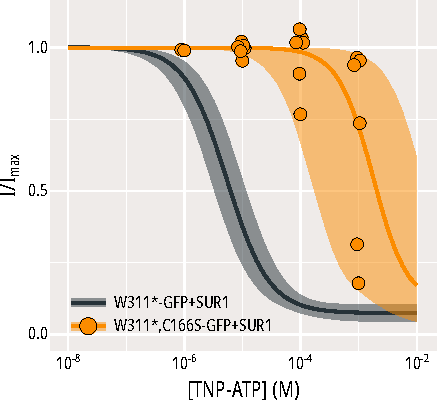
\includegraphics[width=\textwidth]{c166s_7.pdf}
	\end{subfigure}
	\hfill
	\begin{subfigure}[t]{0.6\textwidth}
		\caption{}\label{ch5fig:c166s_params_2}
		\centering
		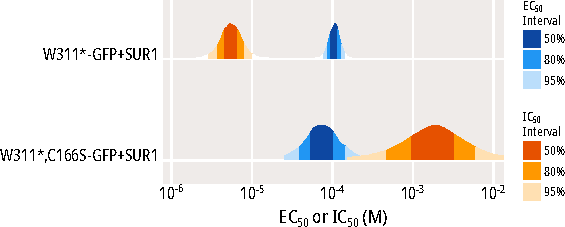
\includegraphics[width=\textwidth]{c166s_8.pdf}
	\end{subfigure}
	\vfill
	\begin{subfigure}[t]{0.9\textwidth}
		\caption{}\label{ch5fig:c166s_indfits_2}
		\centering
		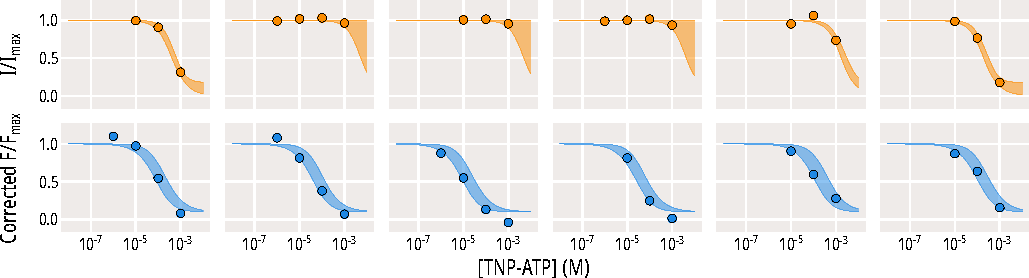
\includegraphics[width=\textwidth]{c166s_9.pdf}
	\end{subfigure}
	\caption[C166S alters sensitivity to nucleotide inhibition]{
	\subref{ch5fig:c166s_traces} Current inhibition (left) and fluorescence quenching (right) from an excised patch expressing W311*,C166S-GFP+SUR1.
	The concentration of TNP-ATP perfused is shown by colour.
	The location of the peak ANAP fluorescence is marked as a grey box.
	\subref{ch5fig:c166s_popfits_2} Fluorescence quenching of W311*,C166S-GFP+SUR1 by TNP-ATP in excised patches.
	Each point represents an individual experiment.
	The smooth filled curves are the \SI{95}{\percent} intervals of the posterior probability distribution of fits to equation \ref{eq:hill} as described in the methods.
	\subref{ch5fig:c166s_popfits_3} Current inhibition of W311*,C166S-GFP+SUR1 by TNP-ATP in excised patches.
	Each point represents an individual experiment.
	The smooth filled curves are the \SI{95}{\percent} intervals of the posterior probability distribution of fits to equation \ref{eq:hill} as described in the methods.
	\subref{ch5fig:c166s_params_2} Posterior probability distributions for the estimated population EC\textsubscript{50} (blue) and IC\textsubscript{50} (orange) values are shown shaded according to their intervals.
	\subref{ch5fig:c166s_indfits_2} Data from each experiment is shown separately; each column represents one excised patch..
	The smooth filled curves are the \SI{95}{\percent} intervals of the posterior predictions for each experiment.
	}\label{ch5fig:c166s_2}
\end{figure}

Fitting our data to the MWC-type model described previously, we found that in addition to the effects of the C166S mutation on the intrinsic open probability of K\ATP{}, there is a striking shift in $D$ (Figure \ref{ch5fig:c166s_mwc_params_1}).
This shift to a value much closer to unity indicates that binding of TNP-ATP to W311*,C166S-GFP+SUR1 favours the closed state far less than binding of TNP-ATP to W311*-GFP+SUR1.
Equivalently, binding of TNP-ATP to the mutant channel is less able to induce closure of the pore.
Thus, even at millimolar concentrations of TNP-ATP when all of the Kir6.2 subunits are predicted to be bound, the K\ATP{} channels are still able to open.

\begin{figure}[h]
	\centering
	\begin{subfigure}[t]{0.9\textwidth}
		\caption{}\label{ch5fig:c166s_mwc_params_1}
		\centering
		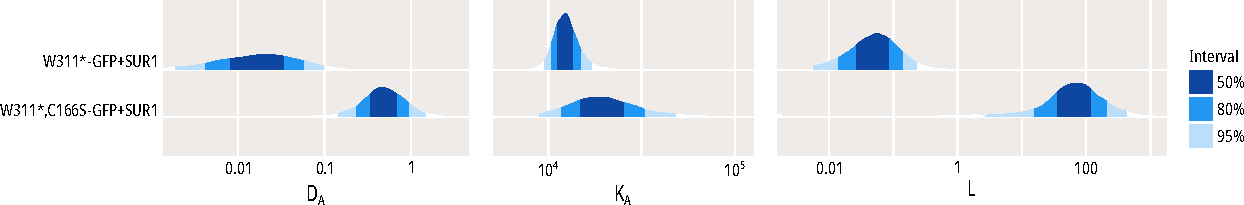
\includegraphics[width=\textwidth]{mwc_c166s_2.pdf}
	\end{subfigure}
	\vfill
	\begin{subfigure}[t]{0.45\textwidth}
		\caption{}\label{ch5fig:c166s_mwc_params_2}
		\centering
		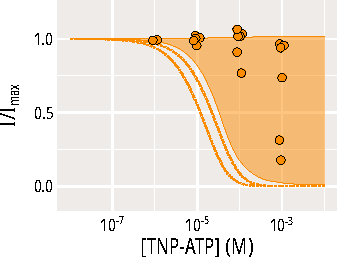
\includegraphics[width=\textwidth]{mwc_c166s_3.pdf}
	\end{subfigure}
	\hfill
	\begin{subfigure}[t]{0.45\textwidth}
		\caption{}\label{ch5fig:tea_trace}
		\centering
		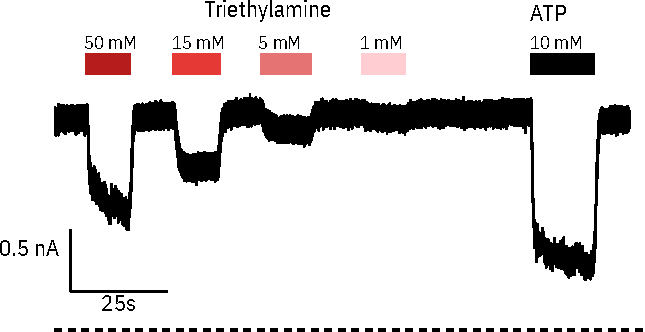
\includegraphics[width=\textwidth]{tea_trace.pdf}
	\end{subfigure}
	\vfill
	\begin{subfigure}[t]{0.45\textwidth}
		\caption{}\label{ch5fig:tea_drc}
		\centering
		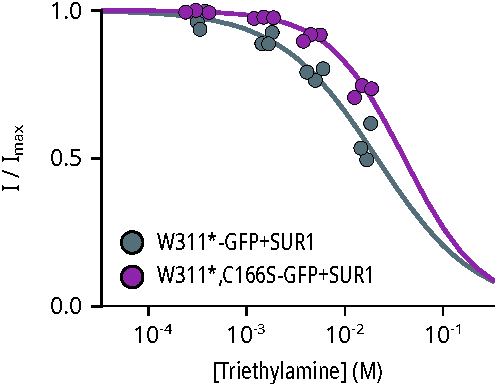
\includegraphics[width=\textwidth]{tea_drc.pdf}
	\end{subfigure}
	\hfill
	\begin{subfigure}[t]{0.45\textwidth}
		\caption{}\label{ch5fig:l_d_sim}
		\centering
		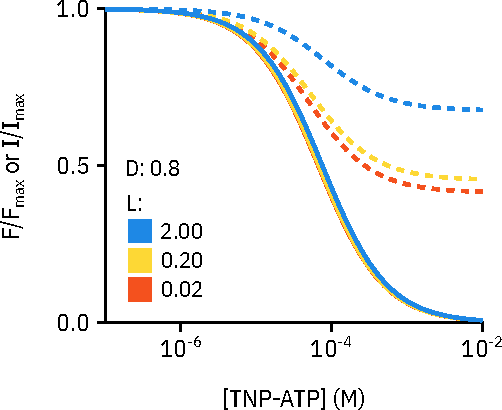
\includegraphics[width=\textwidth]{c166s_param_sim_1.pdf}
	\end{subfigure}
	\caption[C166S alters transduction of nucleotide binding to Kir6.2]{
	}\label{ch5fig:c166s_3}
\end{figure}

This finding makes the prediction that nucleotide inhibition of K\ATP{} channels with the C166S mutation will exhibit a plateau of inhibition.
Unfortunately, we were not able to test this directly with higher concentrations of TNP-ATP due to its purification as a TEA\textsuperscript{+} salt.
High \si{\milli\Molar} concentrations of TEA\textsuperscript{+} inhibit K\ATP{} channels, and we determined that for W311*-GFP+SUR1 and W311*,C166S-GFP+SUR1 concentrations of above \SI{1}{\milli\Molar} TEA\textsuperscript{+} began to inhibit currents to an extent that would interfere with our measurements (Figure \ref{ch5fig:tea_trace}, \ref{ch5fig:tea_drc}).
The precise ratio of TEA\textsuperscript{+} to TNP-ATP in our solutions is unknown, but is assumed to be between 1:1 and 3:1.
Any additional inhibition observed at TNP-ATP concentrations greater than \SI{1}{\milli\Molar} for W311*,C166S-GFP+SUR1 will therefore be (at least in part) due to the presence of TEA\textsuperscript{+}.
However, we do see that even at concentrations of \SI{10}{\milli\Molar} ATP, W311*,C166S-GFP+SUR1 is not fully inhibited (Figure \ref{ch5fig:c166s_mwc_fit_1}, open circle).
The literature is divided on the existence of a current plateau for mutations at C166, although these experiments have been performed under a variety of different conditions and with various different Kir6.2 backgrounds.

\subsection{Mutations at E179 alter both inhibition and binding}

Residue E179 of Kir6.2 is located in the C-terminal region of Kir6.2 between the inhibitory nucleotide binding site and the proposed PIP\textsubscript{2} binding site.
In one early predicted structures of Kir6.2, it was theorised that E179 would form part of the nucleotide binding pocket directly, potentially coordinating the adenine ring of ATP directly through hydrogen bonding \cite{antcliff_functional_2005}.
In another, it was hypothesised to form part of the PIP\textsubscript{2} binding pocket instead \cite{haider_identification_2007}.
Electrophysiological experiments painted a confusing picture of the residues role \cite{antcliff_functional_2005}.
Mutation to an amino acid capable of forming hydrogen bonds (Q) resulted in no change in the IC\textsubscript{50} for nucleotide inhibition (although a separate study found that Q increased the IC\textsubscript{50} \cite{proks_involvement_1999}), while only one of two amino acids incapable of forming hydrogen bonds tested (M and L) resulted in an increased IC\textsubscript{50}.
In addition, mutation of the residue to asparagine (which is not capable of forming hydrogen bonds) not only dramatically increased the nucleotide IC\textsubscript{50}, but increased the intrinsic open probability of the channel \cite{antcliff_functional_2005}.

The cryo-EM structures of K\ATP{} in complex with ATP revealed that bound ATP adopted a radically different conformation to that proposed in early models, and the E179 side chain actually lies over \SI{8}{\angstrom} away from bound ATP \cite{lee_molecular_2017, martin_anti-diabetic_2017, li_structure_2017, puljung_cryo-electron_2018-1}.
Unfortunately, no structure has been resolved in the presence of PIP\textsubscript{2} to date.
However, coarse-grained molecular dynamics simulations using the cryo-EM structures as a starting point indicate that E179 may form part of the PIP\textsubscript{2} binding pocket \cite{pipatpolkai_evaluating_2020}.
In addition, mutation to E179K results in reduced inhibition of the channel by the sequestering agent neomycin - potentially due to an increased affinity of the mutated residue for PIP\textsubscript{2} \cite{pipatpolkai_evaluating_2020}.

To attempt to resolve the precise role of E179 in nucleotide binding and inhibition, we first determined how ATP and TNP-ATP inhibiton of K\ATP{} channels was affected by mutation of E179 to A or K.
For E179A-GFP+SUR1 and E179K-GFP+SUR1, we observed an increase in IC\textsubscript{50} for both ATP and TNP-ATP inhibition.
ATP inhibition did not seem to be influenced by the identity of the replacement amino acid (x and x respectively), while TNP-ATP inhibition was more reduced by mutation to a K rather than an A ( x and x respectively).
Introducing the mutations into the ANAP-labelled construct did not affect the relative changes in inhibition by either nucleotide, with ATP inhibition occurring at similar IC\textsubscript{50}s for A and K (x and x respectively) and with K increasing the IC\textsubscript{50} for TNP-ATP more than A (x and x respectively).
Measurements of TNP-ATP binding mirrored our observations for current inhibition by TNP-ATP, with mutation to both A and K resulting in an increased apparant binding EC\textsubscript{50}, with K having more of an effect than A (x and x respectively).
Fitting the combined data to the MWC-type model, we found that both mutations resulted in a decreased $K_A$ estimate, with no apparent change in $L$.
In addition, mutation to a K led to a $D$ value closer to unity than for E or A.

We believe there are two possible ways to interpret these findings.
The first is to accept the shift in $K_A$ at face value - a decrease in the apparent TNP-ATP binding affinity would suggest a role for residue E179 in forming the nucleotide binding pocket, and this function is abrogated by our mutations.
Despite the distance of the residue from the bound ATP, there could be interactions between E179 and the sidechains of residues which do form the pocket (e.g. R54), such that mutation of E179 leads to alterations in the binding pocket which reduce nucleotide binding affinity and therefore our estimate of $K_A$.
The additional effect on $D$ caused by mutating the residue to K suggests a dysregulation of the transduction of nucleotide binding to the channel pore, making nucleotides less selective for the close state.

The second interpretation is possible due to the simplification of the role of PIP\textsubscript{2} in our MWC model as discussed previously.
Briefly, if there is an additional allosteric interaction between nucleotide and PIP\textsubscript{2} binding to Kir6.2 which is separate to the channels open/closed state, then changes in $K_A$ may reflect alterations in the affinity for PIP\textsubscript{2} binding in addition to or instead of alterations in the affinity for nucleotide binding.
Thus, the decrease in $K_A$ upon mutation of E179 may reflect an increase in PIP\textsubscript{2} affinity and demonstrate the presence of local allostery between nucleotide and lipid.

Distinguishing between these two interpretations is difficult given our current evidence, and essentially depends on the weight you place on the assumptions of each, but should be possible with one or two further experiments.
Firstly, an increase in PIP\textsubscript{2} affinity should lead to an increase in channel open probability on excision (barring an effect on the relative preference of PIP\textsubscript{2} for the open state).
Our inability to accurately determine the open probability of the macroscopic experiments described so far could be supplemented by single channel analysis of the mutants to test this directly.
In addition, we could measure the affinity of PIP\textsubscript{2} directly in macroscopic patches.
Finally, to definitively test the existence of local allostery between the nucleotide and PIP\textsubscript{2} binding sites, we could introduce PIP\textsubscript{2} binding mutants into the C166S background.
C166S channels exhibit almost no nucleotide-dependent gating; i.e. nucleotide binding is uncoupled from gating of the channel pore.
Thus, any changes observed in nucleotide binding in the C166S background when PIP\textsubscript{2} affinity is changed must be due to a local allosteric interaction which does not involve the pore.

\subsection{Mutations at K39 alter both inhibition and binding}

Residue K39 of Kir6.2 is located in the N-terminal region of Kir6.2, and is positioned between the inhibitory nucleotide binding site and the proposed PIP\textsubscript{2} binding site.
In previous studies, the mutation K39A has shown a small reduction in open probability \cite{cukras_role_2002}, and a small reduction in sensitivity to nucleotide inhibition \cite{cukras_role_2002, tucker_molecular_1998}.
These effects are somewhat contradictory, as mutations which reduce open probability tend also to increase sensitivity to nucleotide inhibition.
In each of the cryo-EM structures of K\ATP{}, the K39 side chain appears to coordinate the bound ATP molecule \cite{lee_molecular_2017, martin_anti-diabetic_2017, li_structure_2017, puljung_cryo-electron_2018-1}.
These structures are presumed to represent the closed state of the channel, and no PIP\textsubscript{2} bound structure of the channel has yet been solved.
However, molecular dynamics simulations using the ATP-bound structure as a starting point and introducing PIP\textsubscript{2} suggest that the K39 residue is able to contact both ligands.
This suggests a role for K39 in the binding sites of both ATP and PIP\textsubscript{2}, which may explain the contradictory findings on open probability and nucleotide inhibition changes when the residue is mutated.

We tested three mutations at K39 (K39A, K39E, K39R) to examine the effects of changing the side chain characteristics on nucleotide binding and inhibition.
Mutation to E (opposite charge) or R (same charge) results in an increase in IC\textsubscript{50} for ATP inhibition for both WT and W311* backgrounds (x for each).
We did not see an increase in the IC\textsubscript{50} for ATP inhibition when K39 was mutated to A (neutral) in either background (x and x respectively).
Inhibition by TNP-ATP displayed a different profile depending on the mutant residue.
In both WT and W311* backgrounds, inhibition by TNP-ATP exhibited higher IC\textsubscript{50} values for K39A and K39E than we observed for K39R, which was not really distinguishable from K39 (x for each).
Our docked conformation for TNP-ATP suggests that the TNP-moiety of the nucleotide may result in extra contacts with K39 compared to ATP, which may be the cause of the different sensitivity to inhibition between the two nucleotides when this residue is mutated.
Measurements of TNP-ATP binding showed increases in the EC\textsubscript{50} estimates for each of the three mutations (x for each).

Fits of the combined data to the MWC model gave parameter estimates for $K_A$ that decreased from K>R>E>A.
In addition, mutation to an E or an A resulted in $D$ values closer to unity.
Interpretation of these parameters for the R and A mutations is frustrated by the differences in inhibition between TNP-ATP and ATP; we cannot be sure that these differences in binding and inhibition are due to the identity of the nucleotide rather than the identity of the residue.
However, the K39E mutation displayed similar inhibition for both TNP-ATP and ATP.
The increase in our estimate for $D$ when K39 is mutated to an A or an E, but not for R, may indicate a positive charge at the sidechain of this residue being important for transduction of nucleotide binding to the channel pore.


\section{Discussion}